\documentclass{article}

% ready for submission
% \usepackage{neurips_2023}

% to compile a preprint version, e.g., for submission to arXiv, add add the
% [preprint] option:
\usepackage[preprint]{neurips_2023}

% to compile a camera-ready version, add the [final] option, e.g.:
%     \usepackage[final]{neurips_2023}

\usepackage[utf8]{inputenc} % allow utf-8 input
\usepackage[T1]{fontenc}    % use 8-bit T1 fonts
\usepackage{hyperref}       % hyperlinks
\usepackage{url}            % simple URL typesetting
\usepackage{booktabs}       % professional-quality tables
\usepackage{amsfonts}       % blackboard math symbols
\usepackage{nicefrac}       % compact symbols for 1/2, etc.
\usepackage{microtype}      % microtypography
\usepackage{xcolor}         % colors
\usepackage{graphicx}       % figures

\graphicspath{ {figures/} }

\title{QwinSR: An All-MLP Shifted Window Model for Image Super Resolution}

\author{
  Mark Bauer\thanks{Use footnote for providing further information
    about author (webpage, alternative address)---\emph{not} for acknowledging
    funding agencies.} \\
  Siebel Department of Computer Science\\
  University of Illinois Urbana-Champaign\\
  \texttt{markb6@illinois.edu} \\
  \And
  Quinn Ouyang\thanks{"Quinn" $=$ "Qwin"} \\
  School of Music \\
  University of Illinois Urbana-Champaign \\
  \texttt{qouyang3@illinois.edu} \\
}

\begin{document}

\maketitle

\begin{abstract}
    Since its inception, the Swin Transformer backbone architecture has consistently showcased remarkable performance across a range of well-established computer vision benchmarks. To enhance computational efficiency, the Swin Mixer architecture has adopted a similar structure. However, it distinguishes itself by substituting transformers with Mixer Layers, thus giving rise to Swin Mixer Layers (SMLs). In line with this design, we introduce QwinSR, an application of this all-MLP architecture tailored for the task of single image super-resolution. This adaptation simplifies the original transformer-based image restoration model, SwinIR. QwinSR leverages SMLs to extract essential features and subsequently aggregates them within a compact convolutional neural network, facilitating image reconstruction. We anticipate that this approach will yield competitive accuracy-to-computation ratios, particularly when compared to SwinIR and other leading models in the field.
\end{abstract}

\section{Introduction}

Despite advances in modern photography and image transmission technology, resolution loss is often an unavoidable or necessary compromise. This produces a need and desire for techniques to construct higher fidelity images from lower resolution sources, which we call super resolution (SR) imaging. However, SR is a more niche category than other computer vision tasks (such as classification and semantic segmentation []), making this field ripe for new research. Given the simple objective and need for research on SR, we propose a simplified all-MLP model based on the shifted window design from Swin Transformer: QwinIR.

\subsection{Related Work}

\subsubsection{Single Image Super-Resolution}

“Super-resolution” generally refers to the process of enhancing the visual detail and fidelity of an image by predicting pixels to increase its resolution []. In other literature, SR is roughly interchangeable with the more general terms “upsampling” and “reconstruction.” Note that the latter implies that an exact / true higher resolution image exists for a lower resolution one, which typically comes from artificial downsampling (classic image SR) []. “Single image”  differentiates from the other common variant of this task, multiple image SR, which assumes the advantage of having more than one source image. Effective techniques exploit the related images for more pixel information to construct from, which can apply in the real-world (e.g. a burst shot, video frames, etc.) []. However, we focus on single image SR as it is a more fundamental and challenging task.

Traditional algorithmic approaches for SR directly interpolate pixels from a lower resolution source, typically assuming a downsampling process to generalize the reconstruction. Popular basic algorithms include bicubic and nearest-neighbor interpolation which are fast and eschew the long training times associated with learning-based models, but the absence of trained priors obviously limits their ability to hallucinate new pixels [].

\subsubsection{Learning-based Approaches}

On the other hand, learning-based models spanning a variety of architectures have far surpassed the generalized interpolations that traditional approaches limit themselves to [], as we have briefly illustrated in Figure~\ref{fig:example}. Models based on convolutional neural networks (e.g. SRCNN, SRResNet), general adversarial networks (e.g. ESRGAN, SRGAN, Real-ESRGAN), and transformers (e.g. SwinIR) have all effectively competed for state-of-the-art performance [].

\begin{figure}
    \centering
    \begin{tabular}{c c c c}
        
\includegraphics[width=80pt]{bicubic.png} & 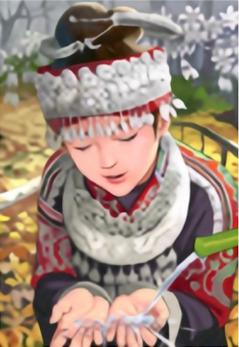
\includegraphics[width=80pt]{srresnet.png} & 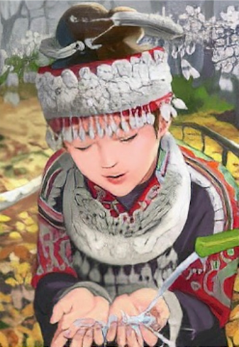
\includegraphics[width=80pt]{srgan.png} & 
\includegraphics[width=80pt]{original.png} \\
        \small Bicubic Interpolation              & \small SRResNet                            & \small SRGAN                            & \small Original
    \end{tabular}

    \caption{Visual comparisons of traditional and learning-based classic image SR approaches to a $\times 4$-upscaled original high resolution image.}\label{fig:example}
\end{figure}

For SR related tasks, CNNs are effective at global feature extraction but have lately been usurped by transformers, which tend to be more robust and lightweight. As a consequence, pure CNN models often require added complexity just to match the performance of transformer models [https://arxiv.org/pdf/2105.01601.pdf]. It is quite common to utilize hybrid CNN-transformer models, in which CNNs are used for global feature extraction while transformers focus on local feature extraction []. E.g. …

GANs tend to be tedious to fine tune and also have many trainable parameters, making the training process very long []. Similarly, diffusion models like StableSR have gigantic datasets and are quite complex []. The focus of this research project is on simplicity, and as such we do not consider these models.

% ~~~ NEURIPS NOTES ~~~

\section{Citations, figures, tables, references}
\label{others}


These instructions apply to everyone.


\subsection{Citations within the text}


The \verb+natbib+ package will be loaded for you by default.  Citations may be
author/year or numeric, as long as you maintain internal consistency.  As to the
format of the references themselves, any style is acceptable as long as it is
used consistently.


The documentation for \verb+natbib+ may be found at
\begin{center}
    \url{http://mirrors.ctan.org/macros/latex/contrib/natbib/natnotes.pdf}
\end{center}
Of note is the command \verb+\citet+, which produces citations appropriate for
use in inline text.  For example,
\begin{verbatim}
   \citet{hasselmo} investigated\dots
\end{verbatim}
produces
\begin{quote}
    Hasselmo, et al.\ (1995) investigated\dots
\end{quote}


If you wish to load the \verb+natbib+ package with options, you may add the
following before loading the \verb+neurips_2023+ package:
\begin{verbatim}
   \PassOptionsToPackage{options}{natbib}
\end{verbatim}


If \verb+natbib+ clashes with another package you load, you can add the optional
argument \verb+nonatbib+ when loading the style file:
\begin{verbatim}
   \usepackage[nonatbib]{neurips_2023}
\end{verbatim}


As submission is double blind, refer to your own published work in the third
person. That is, use ``In the previous work of Jones et al.\ [4],'' not ``In our
previous work [4].'' If you cite your other papers that are not widely available
(e.g., a journal paper under review), use anonymous author names in the
citation, e.g., an author of the form ``A.\ Anonymous'' and include a copy of the anonymized paper in the supplementary material.


\subsection{Footnotes}


Footnotes should be used sparingly.  If you do require a footnote, indicate
footnotes with a number\footnote{Sample of the first footnote.} in the
text. Place the footnotes at the bottom of the page on which they appear.
Precede the footnote with a horizontal rule of 2~inches (12~picas).


Note that footnotes are properly typeset \emph{after} punctuation
marks.\footnote{As in this example.}


\subsection{Figures}


\begin{figure}
    \centering
    \fbox{\rule[-.5cm]{0cm}{4cm} \rule[-.5cm]{4cm}{0cm}}
    \caption{Sample figure caption.}
\end{figure}


All artwork must be neat, clean, and legible. Lines should be dark enough for
purposes of reproduction. The figure number and caption always appear after the
figure. Place one line space before the figure caption and one line space after
the figure. The figure caption should be lower case (except for first word and
proper nouns); figures are numbered consecutively.


You may use color figures.  However, it is best for the figure captions and the
paper body to be legible if the paper is printed in either black/white or in
color.


\subsection{Tables}


All tables must be centered, neat, clean and legible.  The table number and
title always appear before the table.  See Table~\ref{sample-table}.


Place one line space before the table title, one line space after the
table title, and one line space after the table. The table title must
be lower case (except for first word and proper nouns); tables are
numbered consecutively.


Note that publication-quality tables \emph{do not contain vertical rules.} We
strongly suggest the use of the \verb+booktabs+ package, which allows for
typesetting high-quality, professional tables:
\begin{center}
    \url{https://www.ctan.org/pkg/booktabs}
\end{center}
This package was used to typeset Table~\ref{sample-table}.


\begin{table}
    \caption{Sample table title}
    \label{sample-table}
    \centering
    \begin{tabular}{lll}
        \toprule
        \multicolumn{2}{c}{Part}                   \\
        \cmidrule(r){1-2}
        Name     & Description     & Size ($\mu$m) \\
        \midrule
        Dendrite & Input terminal  & $\sim$100     \\
        Axon     & Output terminal & $\sim$10      \\
        Soma     & Cell body       & up to $10^6$  \\
        \bottomrule
    \end{tabular}
\end{table}

\subsection{Math}
Note that display math in bare TeX commands will not create correct line numbers for submission. Please use LaTeX (or AMSTeX) commands for unnumbered display math. (You really shouldn't be using \$\$ anyway; see \url{https://tex.stackexchange.com/questions/503/why-is-preferable-to} and \url{https://tex.stackexchange.com/questions/40492/what-are-the-differences-between-align-equation-and-displaymath} for more information.)

\subsection{Final instructions}

Do not change any aspects of the formatting parameters in the style files.  In
particular, do not modify the width or length of the rectangle the text should
fit into, and do not change font sizes (except perhaps in the
\textbf{References} section; see below). Please note that pages should be
numbered.


\section{Preparing PDF files}


Please prepare submission files with paper size ``US Letter,'' and not, for
example, ``A4.''


Fonts were the main cause of problems in the past years. Your PDF file must only
contain Type 1 or Embedded TrueType fonts. Here are a few instructions to
achieve this.


\begin{itemize}


    \item You should directly generate PDF files using \verb+pdflatex+.


    \item You can check which fonts a PDF files uses.  In Acrobat Reader, select the
          menu Files$>$Document Properties$>$Fonts and select Show All Fonts. You can
          also use the program \verb+pdffonts+ which comes with \verb+xpdf+ and is
          available out-of-the-box on most Linux machines.


    \item \verb+xfig+ "patterned" shapes are implemented with bitmap fonts.  Use
          "solid" shapes instead.


    \item The \verb+\bbold+ package almost always uses bitmap fonts.  You should use
          the equivalent AMS Fonts:
          \begin{verbatim}
   \usepackage{amsfonts}
\end{verbatim}
          followed by, e.g., \verb+\mathbb{R}+, \verb+\mathbb{N}+, or \verb+\mathbb{C}+
          for $\mathbb{R}$, $\mathbb{N}$ or $\mathbb{C}$.  You can also use the following
          workaround for reals, natural and complex:
          \begin{verbatim}
   \newcommand{\RR}{I\!\!R} %real numbers
   \newcommand{\Nat}{I\!\!N} %natural numbers
   \newcommand{\CC}{I\!\!\!\!C} %complex numbers
\end{verbatim}
          Note that \verb+amsfonts+ is automatically loaded by the \verb+amssymb+ package.


\end{itemize}


If your file contains type 3 fonts or non embedded TrueType fonts, we will ask
you to fix it.


\subsection{Margins in \LaTeX{}}


Most of the margin problems come from figures positioned by hand using
\verb+\special+ or other commands. We suggest using the command
\verb+\includegraphics+ from the \verb+graphicx+ package. Always specify the
figure width as a multiple of the line width as in the example below:
\begin{verbatim}
   \usepackage[pdftex]{graphicx} ...
   \includegraphics[width=0.8\linewidth]{myfile.pdf}
\end{verbatim}
See Section 4.4 in the graphics bundle documentation
(\url{http://mirrors.ctan.org/macros/latex/required/graphics/grfguide.pdf})


A number of width problems arise when \LaTeX{} cannot properly hyphenate a
line. Please give LaTeX hyphenation hints using the \verb+\-+ command when
necessary.


\begin{ack}
    Use unnumbered first level headings for the acknowledgments. All acknowledgments
    go at the end of the paper before the list of references. Moreover, you are required to declare
    funding (financial activities supporting the submitted work) and competing interests (related financial activities outside the submitted work).
    More information about this disclosure can be found at: \url{https://neurips.cc/Conferences/2023/PaperInformation/FundingDisclosure}.


    Do {\bf not} include this section in the anonymized submission, only in the final paper. You can use the \texttt{ack} environment provided in the style file to autmoatically hide this section in the anonymized submission.
\end{ack}



\section{Supplementary Material}

Authors may wish to optionally include extra information (complete proofs, additional experiments and plots) in the appendix. All such materials should be part of the supplemental material (submitted separately) and should NOT be included in the main submission.


\section*{References}


References follow the acknowledgments in the camera-ready paper. Use unnumbered first-level heading for
the references. Any choice of citation style is acceptable as long as you are
consistent. It is permissible to reduce the font size to \verb+small+ (9 point)
when listing the references.
Note that the Reference section does not count towards the page limit.
\medskip


{
\small


[1] Alexander, J.A.\ \& Mozer, M.C.\ (1995) Template-based algorithms for
connectionist rule extraction. In G.\ Tesauro, D.S.\ Touretzky and T.K.\ Leen
(eds.), {\it Advances in Neural Information Processing Systems 7},
pp.\ 609--616. Cambridge, MA: MIT Press.


    [2] Bower, J.M.\ \& Beeman, D.\ (1995) {\it The Book of GENESIS: Exploring
        Realistic Neural Models with the GEneral NEural SImulation System.}  New York:
TELOS/Springer--Verlag.


[3] Hasselmo, M.E., Schnell, E.\ \& Barkai, E.\ (1995) Dynamics of learning and
recall at excitatory recurrent synapses and cholinergic modulation in rat
hippocampal region CA3. {\it Journal of Neuroscience} {\bf 15}(7):5249-5262.
}

%%%%%%%%%%%%%%%%%%%%%%%%%%%%%%%%%%%%%%%%%%%%%%%%%%%%%%%%%%%%


\end{document}